\documentclass[12pt,a4paper]{article}
\usepackage[margin=1in]{geometry}
\usepackage{ctex}
\usepackage{booktabs}
\usepackage{graphicx}
\usepackage{amsmath}
\usepackage{multirow}
\usepackage{float}
\usepackage{hyperref}
\usepackage{enumitem}
\usepackage{setspace}
\usepackage{adjustbox}
\usepackage[backend=biber,style=gb7714-2015]{biblatex}

\hypersetup{colorlinks=true,linkcolor=blue,citecolor=blue,urlcolor=blue}

% 方正小标宋简体（封面专用）
\newCJKfontfamily\xiaobiaosong{STZhongsong}

\title{\heiti\zihao{3} 集成学习下基于分子指纹的抗癌药物筛选、分析和初步预测}
\author{\songti\zihao{4} 孙睿韩，杨小洋†，李梓旭†}
\date{2026年4月}
\begin{document}
% ================================================================
%  封面
% ================================================================
\newgeometry{top=2.54cm,bottom=2.54cm,left=3.17cm,right=3.17cm}
\begin{titlepage}
    % ---- 作品编号（左对齐，黑体，三号）----
    \noindent{\heiti\fontsize{16}{20}\selectfont 作品编号：\underline{\hspace{7cm}}\par}

    \vspace{1.5cm}

    % ---- 大赛主标题（居中，方正小标宋简体，二号，固定行距45磅）----
    {\centering\xiaobiaosong\fontsize{22}{45}\selectfont
    2026年（第十二届）全国大学生统计建模大赛\par}

    % ---- 参赛作品（居中，方正小标宋简体，一号，行距45磅）----
    {\centering\xiaobiaosong\fontsize{26}{45}\selectfont
    参\hspace{1em}赛\hspace{1em}作\hspace{1em}品\par}

    \vfill

    % ---- 四行信息紧贴底端（仿宋GB2312，小二，单倍行距，居中，等宽）----
    \begin{center}
    {\fangsong\fontsize{18}{22}\selectfont
    \setlength{\tabcolsep}{0pt}%
    \begin{tabular}{r@{}p{11.5cm}}
    参赛学校：& 南开大学 \\[2pt]
    论文题目：& 集成学习下基于分子指纹的抗癌药物筛选、分析和初步预测 \\[2pt]
    参赛队员：& 孙睿韩\quad 杨小洋\quad 李梓旭 \\[2pt]
    指导老师：& 韩东啸 \\
    \end{tabular}\par}
    \end{center}
\end{titlepage}
\restoregeometry

\maketitle

\pagenumbering{arabic}

% ================================================================
%  摘要
% ================================================================
\begin{abstract}
抗癌药物的早期筛选是新药研发的关键瓶颈。本文以表皮生长因子受体（EGFR）抑制剂为研究对象，从ChEMBL数据库获取1830个具有IC$_{50}$活性数据的小分子化合物，利用RDKit计算190个分子描述符与2048位Morgan指纹（ECFP4）作为分子表征，经数据清洗、冗余特征去除与Mutual Information特征选择后保留1000维高信息量特征。在此基础上，训练MLP神经网络、随机森林、梯度提升树、支持向量机、Extra Trees和KNN共6种异质基学习器，并通过Stacking与加权Voting两种集成策略进行融合。经RandomizedSearchCV超参数调优后，优化Stacking集成模型在测试集上取得回归$R^2 = 0.631$、$\text{RMSE} = 0.720$，分类$\text{AUC} = 0.934$、准确率$92.9\%$的最佳性能，相比最优单模型分别提升3.2\%和0.6\%。虚拟筛选实验表明，模型能以91.8\%的准确率从测试分子中正确区分活性与非活性化合物。本研究验证了集成学习在基于分子指纹的药物虚拟筛选中的有效性，为抗癌先导化合物的快速发现提供了可行的计算方案。

\noindent\textbf{关键词：} 集成学习；分子指纹；EGFR抑制剂；虚拟筛选；QSAR；Stacking
\end{abstract}

\clearpage
\tableofcontents
\clearpage
\listoftables
\listoffigures

\clearpage

% ================================================================
%  1. 引言
% ================================================================
\section{引言}

癌症是严重威胁人类健康的重大疾病，全球每年新增病例超过1900万例。 在众多药物靶点中，表皮生长因子受体（Epidermal Growth Factor Receptor, EGFR）因其在非小细胞肺癌、乳腺癌等多种肿瘤中的关键调控作用，成为抗癌药物研发的核心靶标。然而传统的药物筛选流程——从先导化合物发现到临床试验——通常耗时10$\sim$15年、耗资数十亿美元，亟需高效的计算辅助手段加速早期筛选。

定量构效关系（Quantitative Structure-Activity Relationship, QSAR）模型是计算药物化学的基础方法，其核心思想是通过分子结构特征预测化合物的生物活性。分子指纹（Molecular Fingerprint）作为一种将分子结构编码为定长比特向量的技术，因其简洁高效而被广泛应用于QSAR建模。其中，Morgan指纹（Extended-Connectivity Fingerprints, ECFP）通过迭代捕获原子邻域的子结构信息，对化学结构差异具有优异的区分能力。

近年来，集成学习（Ensemble Learning）在机器学习竞赛和工业实践中展现出显著的性能优势。Stacking（堆叠泛化）通过多层学习器组合异质模型的互补信息，Voting（投票法）则通过加权聚合多个模型的预测结果以降低方差。已有研究表明，集成方法在药物活性预测中通常优于单一模型。

本文围绕"集成学习下基于分子指纹的抗癌药物筛选"这一主题，构建了从数据采集、特征工程到模型训练与集成优化的完整流程，旨在回答以下问题：（1）分子描述符与Morgan指纹在药物活性预测中的信息贡献如何？（2）Stacking与Voting集成策略能否超越单一机器学习模型？（3）特征选择与超参数调优对集成性能的提升幅度有多大？

% ================================================================
%  2. 数据与方法
% ================================================================
\section{数据与方法}

\subsection{数据来源与预处理}

本研究数据来源于ChEMBL数据库，检索条件为：靶标=EGFR（Target ChEMBL ID: CHEMBL203），活性类型=IC$_{50}$，数据可信度$\geq$9。原始数据集包含3743条记录。数据预处理流程如下：

\begin{enumerate}[leftmargin=2em]
    \item \textbf{缺失值处理}：移除pChEMBL Value缺失的记录；
    \item \textbf{分子去重}：以Molecule ChEMBL ID为唯一标识，对同一分子的多次测量取中位数聚合，得到1830个唯一分子；
    \item \textbf{异常值处理}：移除描述符中的无穷值，将NaN替换为列中位数；
    \item \textbf{零方差特征移除}：删除114个数值恒定的特征列。
\end{enumerate}

最终清洗后的数据集包含1830个分子、2151个特征列。pChEMBL Value（即$-\log_{10}\text{IC}_{50}$，单位M）的统计特征为：均值7.260，标准差1.231，范围$[4.02, 10.19]$。以pChEMBL $\geq 6.0$为阈值将分子标记为活性（Active，1554个，84.9\%）与非活性（Inactive，276个，15.1\%）。

\begin{table}[H]
\centering
\caption{环节1至环节2的数据规模变化（数据收集与清洗）}
\label{tab:phase1_dataflow}
\begin{adjustbox}{max width=\textwidth}
\begin{tabular}{lcc}
\toprule
阶段 & 样本规模 & 说明 \\
\midrule
环节1：原始采集后可用记录 & 3743 & ChEMBL中EGFR靶点且具备有效IC$_{50}$/pChEMBL数据 \\
环节2：按分子去重后唯一分子 & 1830 & 同一分子多次实验记录取中位数聚合 \\
环节2：特征维度 & 2151 & 描述符与Morgan指纹拼接后保留的特征数 \\
\bottomrule
\end{tabular}
\end{adjustbox}
\end{table}

\subsection{分子表征}

采用RDKit化学信息学工具包计算两类分子特征：

\begin{itemize}[leftmargin=2em]
    \item \textbf{分子描述符}（190个）：包括BCUT2D系列（电荷、极性、摩尔折射率）、拓扑指数（BalabanJ、BertzCT、HallKierAlpha）、Lipinski性质（分子量、AlogP、氢键供体/受体数）、SlogP\_VSA/SMR\_VSA/EState\_VSA等分子表面积描述符。
    \item \textbf{Morgan指纹}（2048位）：使用ECFP4算法（半径=2），生成的2048位二值向量中1952位在数据集中具有非零方差而被保留。
\end{itemize}

\subsection{特征工程}

\subsubsection{冗余特征去除}

计算190个描述符的Pearson相关系数矩阵，将$|r| > 0.95$的冗余描述符逐步移除（保留对pChEMBL相关性更高者），最终保留153个描述符。与1952位指纹合并后得到2105维特征向量。

\subsubsection{基于互信息的特征选择}

为进一步降低噪声，使用互信息回归（Mutual Information Regression）评估每个特征对pChEMBL Value的非线性相关性。对$k \in \{200, 500, 800, 1000, 1500, 2105\}$进行快速交叉验证评估，$k = 1000$时Random Forest的5折CV $R^2$最高（0.625），故最终选取MI排名前1000的特征（描述符137个 + 指纹863位）。MI排名前5的特征为：MaxPartialCharge（0.204）、SlogP\_VSA2（0.203）、BCUT2D\_LOGPLOW（0.195）、MinEStateIndex（0.181）、BCUT2D\_CHGHI（0.180）。

\subsubsection{数据划分与标准化}

采用分层抽样按8:1:1比例将数据划分为训练集（1464个）、验证集（183个）和测试集（183个），确保各子集中活性/非活性分子比例一致。对描述符特征进行StandardScaler标准化（$z$-score），Morgan指纹保持原始0/1编码。

\begin{table}[H]
\centering
\caption{环节3：特征工程关键结果汇总}
\label{tab:phase3_feature_engineering}
\begin{tabular}{lc}
\toprule
项目 & 结果 \\
\midrule
描述符初始维度 & 190 \\
高相关冗余剔除后描述符维度 & 153 \\
有效Morgan指纹维度 & 1952 \\
融合后总特征维度 & 2105 \\
互信息筛选后特征维度 & 1000 \\
数据集划分比例（训练/验证/测试） & 8:1:1 \\
\bottomrule
\end{tabular}
\end{table}

\subsection{基学习器}

本文选取以下6种异质机器学习模型作为基学习器：

\begin{enumerate}[leftmargin=2em]
    \item \textbf{MLP神经网络}：3层全连接网络（128-64-32），Adam优化器，自适应学习率，Early Stopping。
    \item \textbf{随机森林（RF）}：674棵决策树，max\_features=0.5，无深度限制。
    \item \textbf{梯度提升树（HGBT）}：等价于XGBoost/LightGBM的sklearn实现，220轮迭代，max\_depth=7，学习率0.075。
    \item \textbf{支持向量机（SVM）}：RBF核函数，$C=4.65$，$\epsilon=0.019$。
    \item \textbf{极端随机树（Extra Trees）}：与RF类似但在分裂点选择上引入更多随机性，降低方差。
    \item \textbf{K近邻（KNN）}：基于距离加权的实例学习方法。
\end{enumerate}

所有模型的超参数通过RandomizedSearchCV在30组随机配置中以5折交叉验证$R^2$为评价指标进行搜索。分类模型对少数类（Inactive）采用class\_weight=``balanced''进行加权补偿。

\subsection{集成策略}

\subsubsection{Stacking（堆叠泛化）}

Stacking通过两层结构实现模型融合：第一层由6个基学习器组成，每个基学习器通过5折交叉验证生成训练集的预测值；第二层元学习器以第一层的6维预测输出为输入进行最终预测。回归任务的元学习器为RidgeCV（$\alpha$从$\{0.001, 0.01, 0.1, 1, 10, 100\}$中自动选择），分类任务为LogisticRegressionCV。

\subsubsection{Voting（加权投票）}

Voting集成对6个基学习器的预测结果进行加权平均。权重按各模型的调优CV $R^2$归一化分配，权重分布为：MLP=0.152, RF=0.169, HGBT=0.166, SVM=0.175, ET=0.178, KNN=0.158。分类任务采用Soft Voting（基于预测概率的加权平均）。

\subsection{评价指标}

\begin{itemize}[leftmargin=2em]
    \item \textbf{回归任务}：决定系数$R^2$、均方根误差RMSE、平均绝对误差MAE。
    \item \textbf{分类任务}：AUC（ROC曲线下面积）、准确率Accuracy、F1分数、精确率Precision、召回率Recall。
    \item \textbf{模型稳定性}：5折交叉验证的均值$\pm$标准差。
\end{itemize}

% ================================================================
%  3. 结果与分析
% ================================================================
\section{结果与分析}

\subsection{探索性数据分析}

pChEMBL Value呈近似正态分布（均值7.26，偏度$-0.24$），主要集中在6.0$\sim$9.0区间。Lipinski五规则分析显示：85.4\%的分子满足分子量$\leq$500, 78.4\%满足AlogP$\leq$5, 96.3\%满足氢键供体$\leq$5, 81.4\%满足氢键受体$\leq$10，表明数据集中的分子大部分具有良好的类药性。

特征相关性分析揭示了分子描述符间的强共线性（如MolWt与HeavyAtomMolWt的$r=0.999$），为特征工程中的冗余去除提供了依据。PCA分析表明前50个主成分解释了约80\%的方差，说明高维特征空间存在显著的信息冗余。

\begin{figure}[H]
\centering
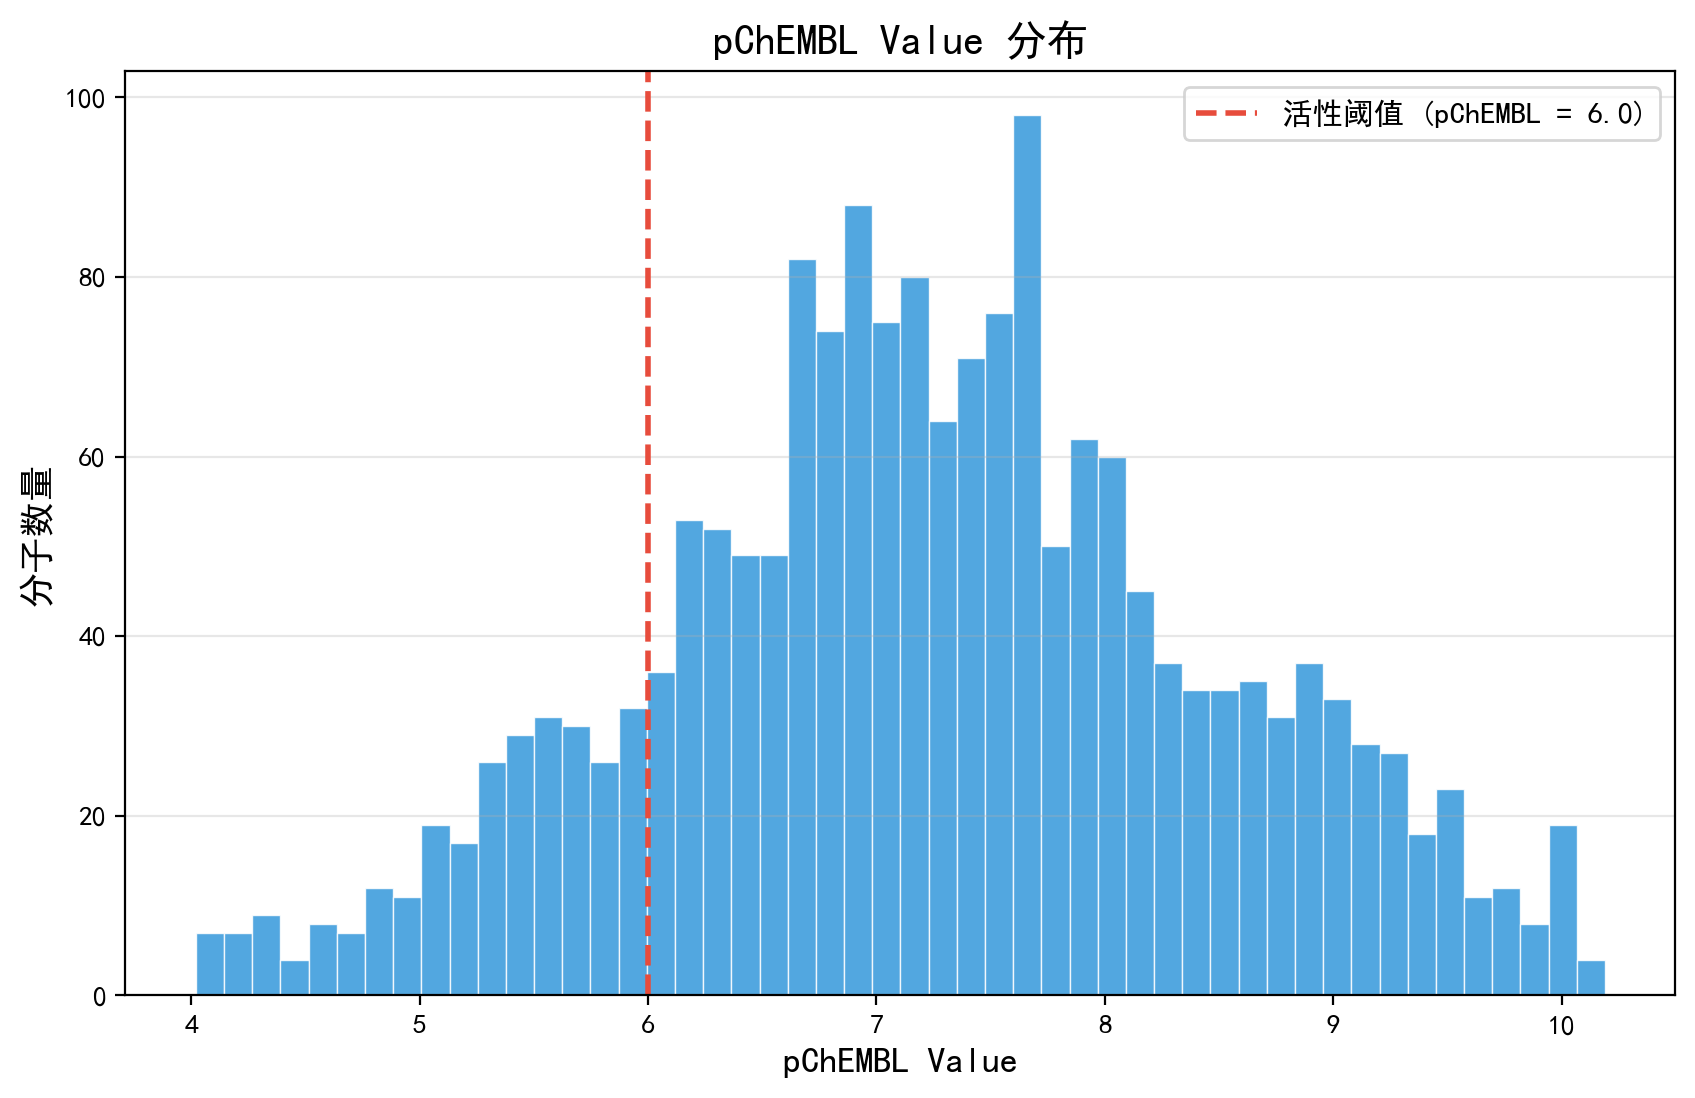
\includegraphics[width=0.72\textwidth]{../环节二：数据清洗与EDA/figures/01_pchembl_distribution.png}
\caption{环节2：pChEMBL活性值分布}
\label{fig:phase2_pchembl_distribution}
\end{figure}

\begin{figure}[H]
\centering
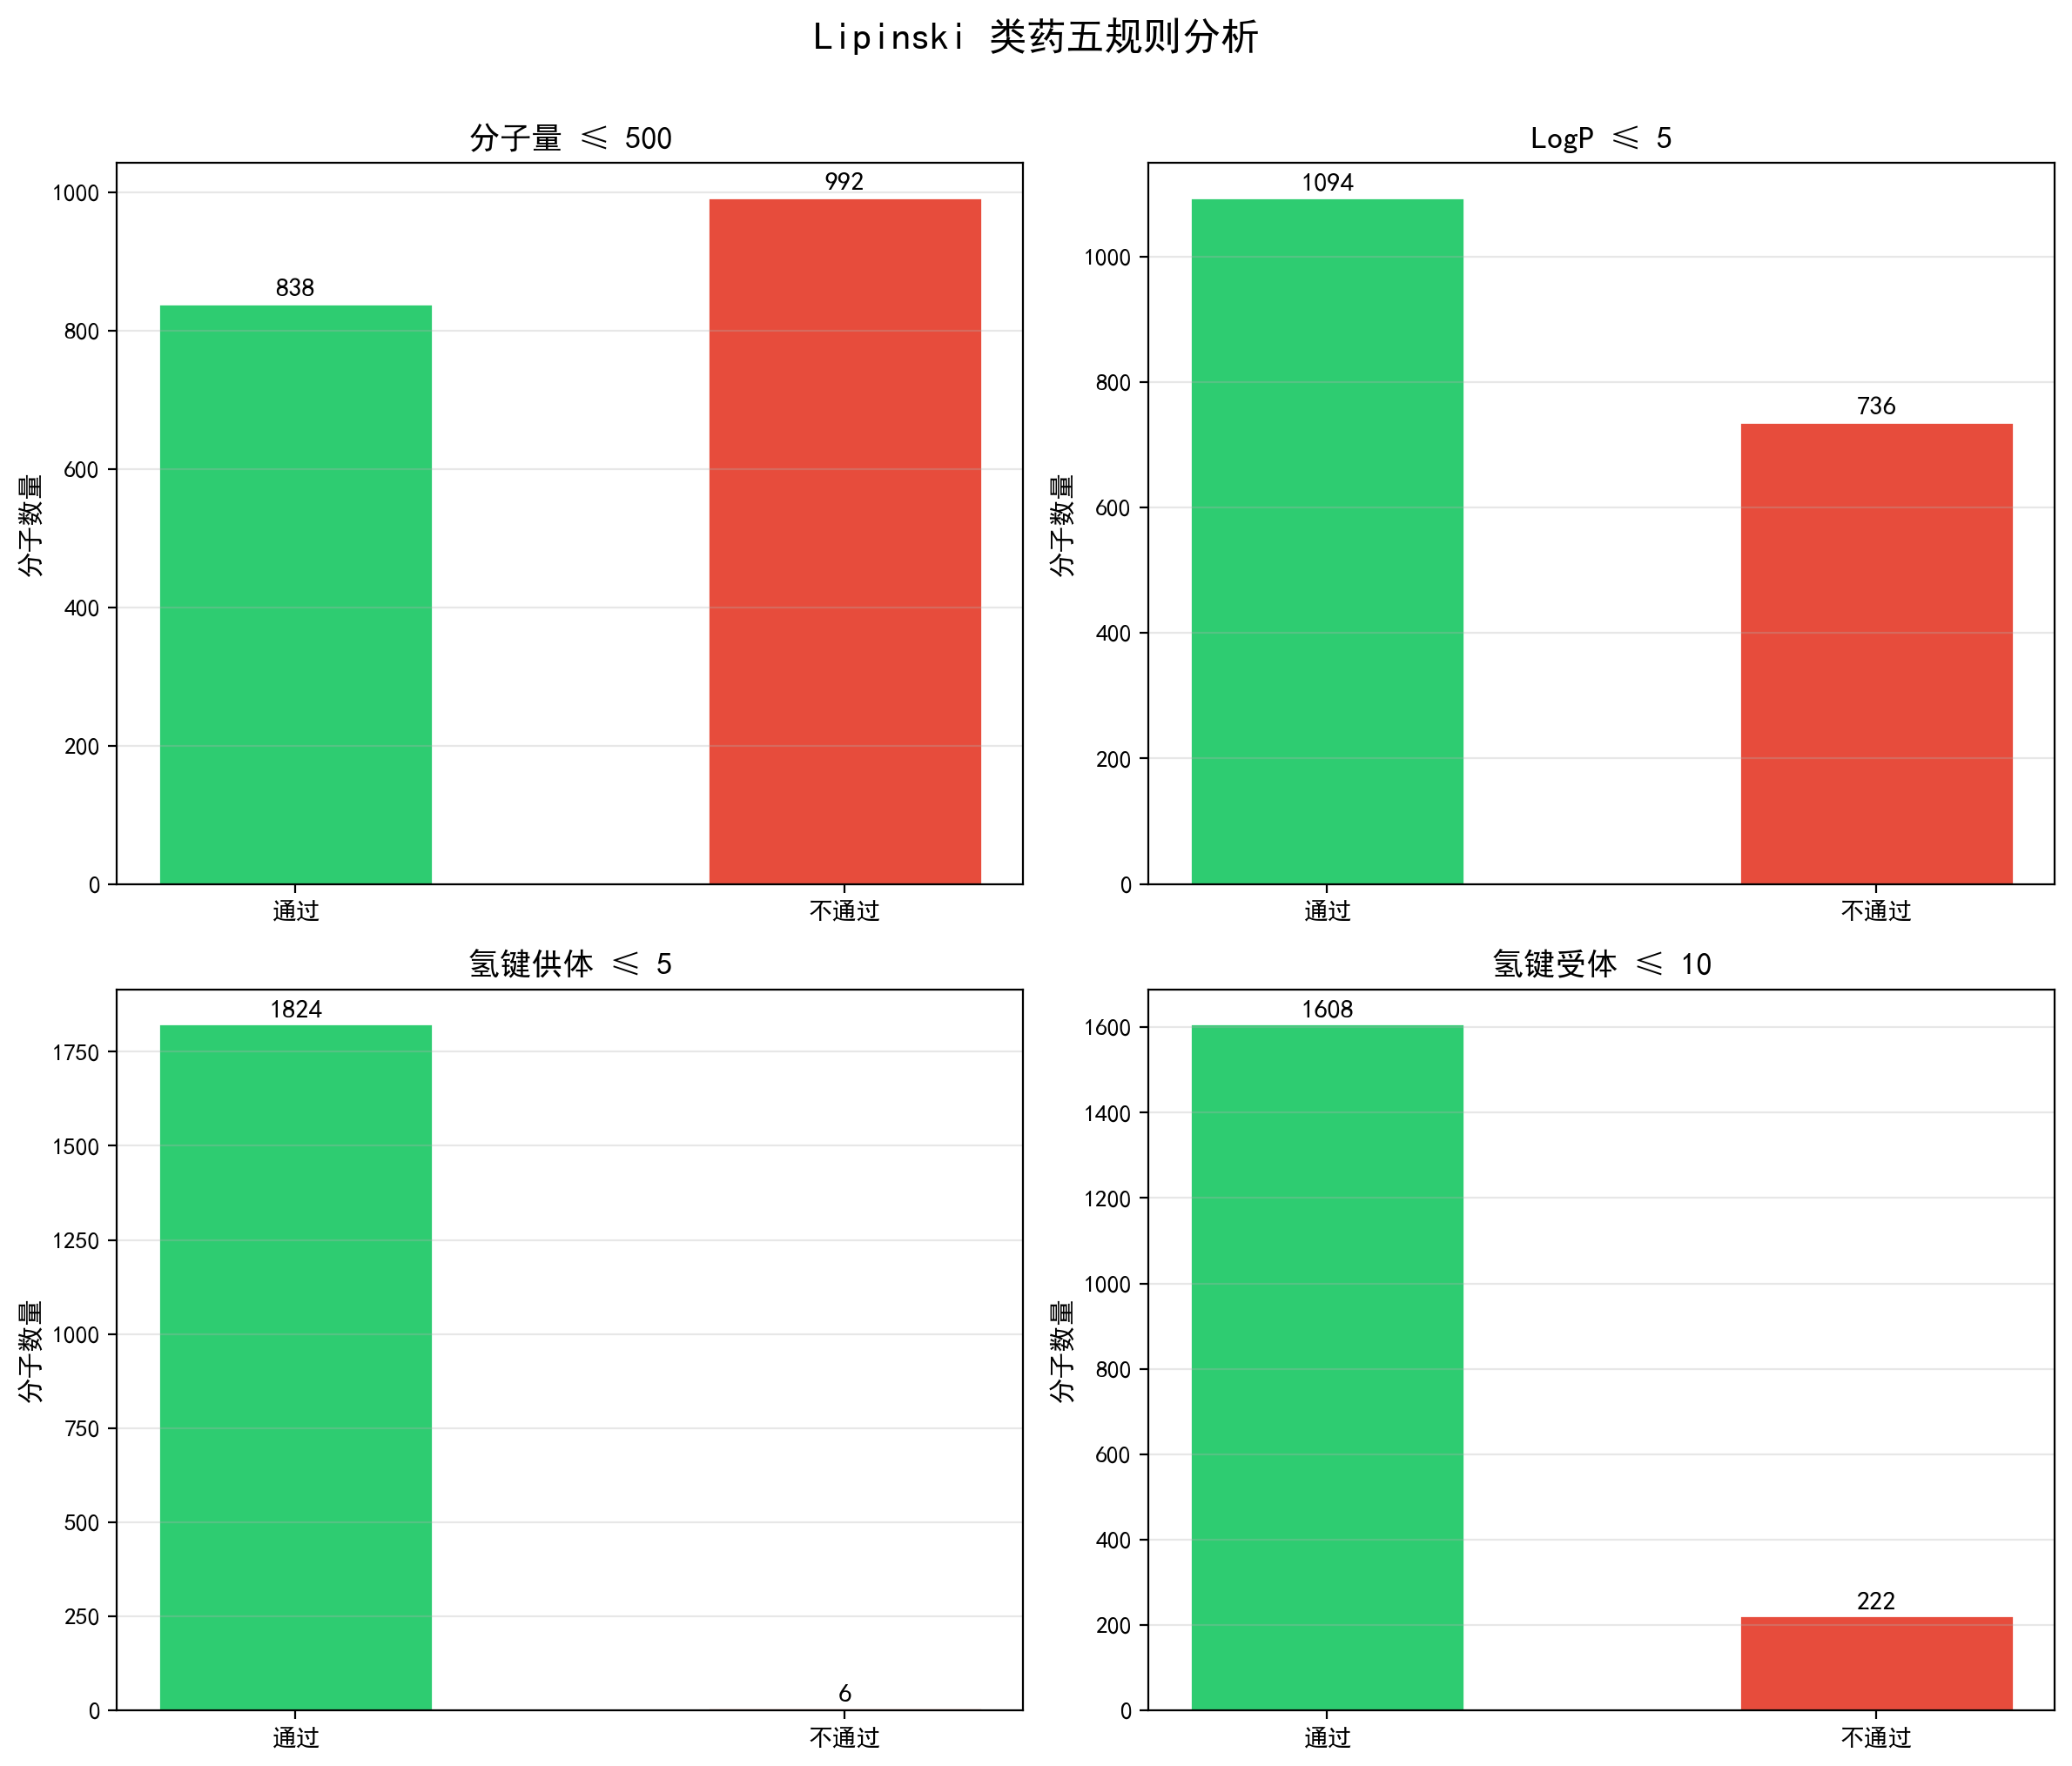
\includegraphics[width=0.72\textwidth]{../环节二：数据清洗与EDA/figures/05_lipinski_rules.png}
\caption{环节2：Lipinski五规则满足情况}
\label{fig:phase2_lipinski}
\end{figure}

\subsection{单模型性能对比}

表\ref{tab:single_reg}和表\ref{tab:single_cls}分别列出了优化前后各单模型在测试集上的回归和分类性能。

\begin{table}[H]
\centering
\caption{回归任务测试集性能（优化前/优化后）}
\label{tab:single_reg}
\begin{adjustbox}{max width=\textwidth}
\begin{tabular}{lcccccc}
\toprule
\multirow{2}{*}{模型} & \multicolumn{3}{c}{优化前} & \multicolumn{3}{c}{优化后} \\
\cmidrule(lr){2-4}\cmidrule(lr){5-7}
 & $R^2$ & RMSE & MAE & $R^2$ & RMSE & MAE \\
\midrule
MLP神经网络 & 0.500 & 0.839 & 0.616 & 0.459 & 0.872 & 0.643 \\
随机森林 & 0.587 & 0.763 & 0.566 & 0.604 & 0.747 & 0.549 \\
梯度提升树 & 0.546 & 0.799 & 0.586 & 0.551 & 0.795 & 0.591 \\
SVM (RBF) & 0.565 & 0.782 & 0.550 & 0.588 & 0.761 & 0.542 \\
Extra Trees & -- & -- & -- & \textbf{0.638} & \textbf{0.713} & \textbf{0.519} \\
KNN & -- & -- & -- & 0.563 & 0.784 & 0.565 \\
\bottomrule
\end{tabular}
\end{adjustbox}
\end{table}

\begin{table}[H]
\centering
\caption{分类任务测试集性能（优化前/优化后）}
\label{tab:single_cls}
\begin{adjustbox}{max width=\textwidth}
\begin{tabular}{lcccccc}
\toprule
\multirow{2}{*}{模型} & \multicolumn{3}{c}{优化前} & \multicolumn{3}{c}{优化后} \\
\cmidrule(lr){2-4}\cmidrule(lr){5-7}
 & AUC & Accuracy & F1 & AUC & Accuracy & F1 \\
\midrule
MLP神经网络 & 0.898 & 0.918 & 0.953 & 0.919 & 0.902 & 0.943 \\
随机森林 & 0.915 & 0.902 & 0.945 & 0.920 & 0.891 & 0.939 \\
梯度提升树 & 0.881 & 0.869 & 0.922 & 0.875 & 0.902 & 0.943 \\
SVM (RBF) & 0.918 & 0.913 & 0.950 & \textbf{0.929} & \textbf{0.929} & \textbf{0.959} \\
Extra Trees & -- & -- & -- & 0.910 & 0.907 & 0.946 \\
KNN & -- & -- & -- & 0.922 & 0.913 & 0.951 \\
\bottomrule
\end{tabular}
\end{adjustbox}
\end{table}

优化后，随机森林的回归$R^2$从0.587提升至0.604（+0.017），SVM的从0.565提升至0.588（+0.023）。新增的Extra Trees在回归任务中成为最强单模型（$R^2=0.638$），这得益于其在分裂点选择上引入的额外随机性，有效缓解了过拟合。MLP在优化后反而略有下降，可能与特征维度的大幅缩减（2105$\to$1000）导致高维稀疏指纹信息损失有关。

\begin{figure}[H]
\centering
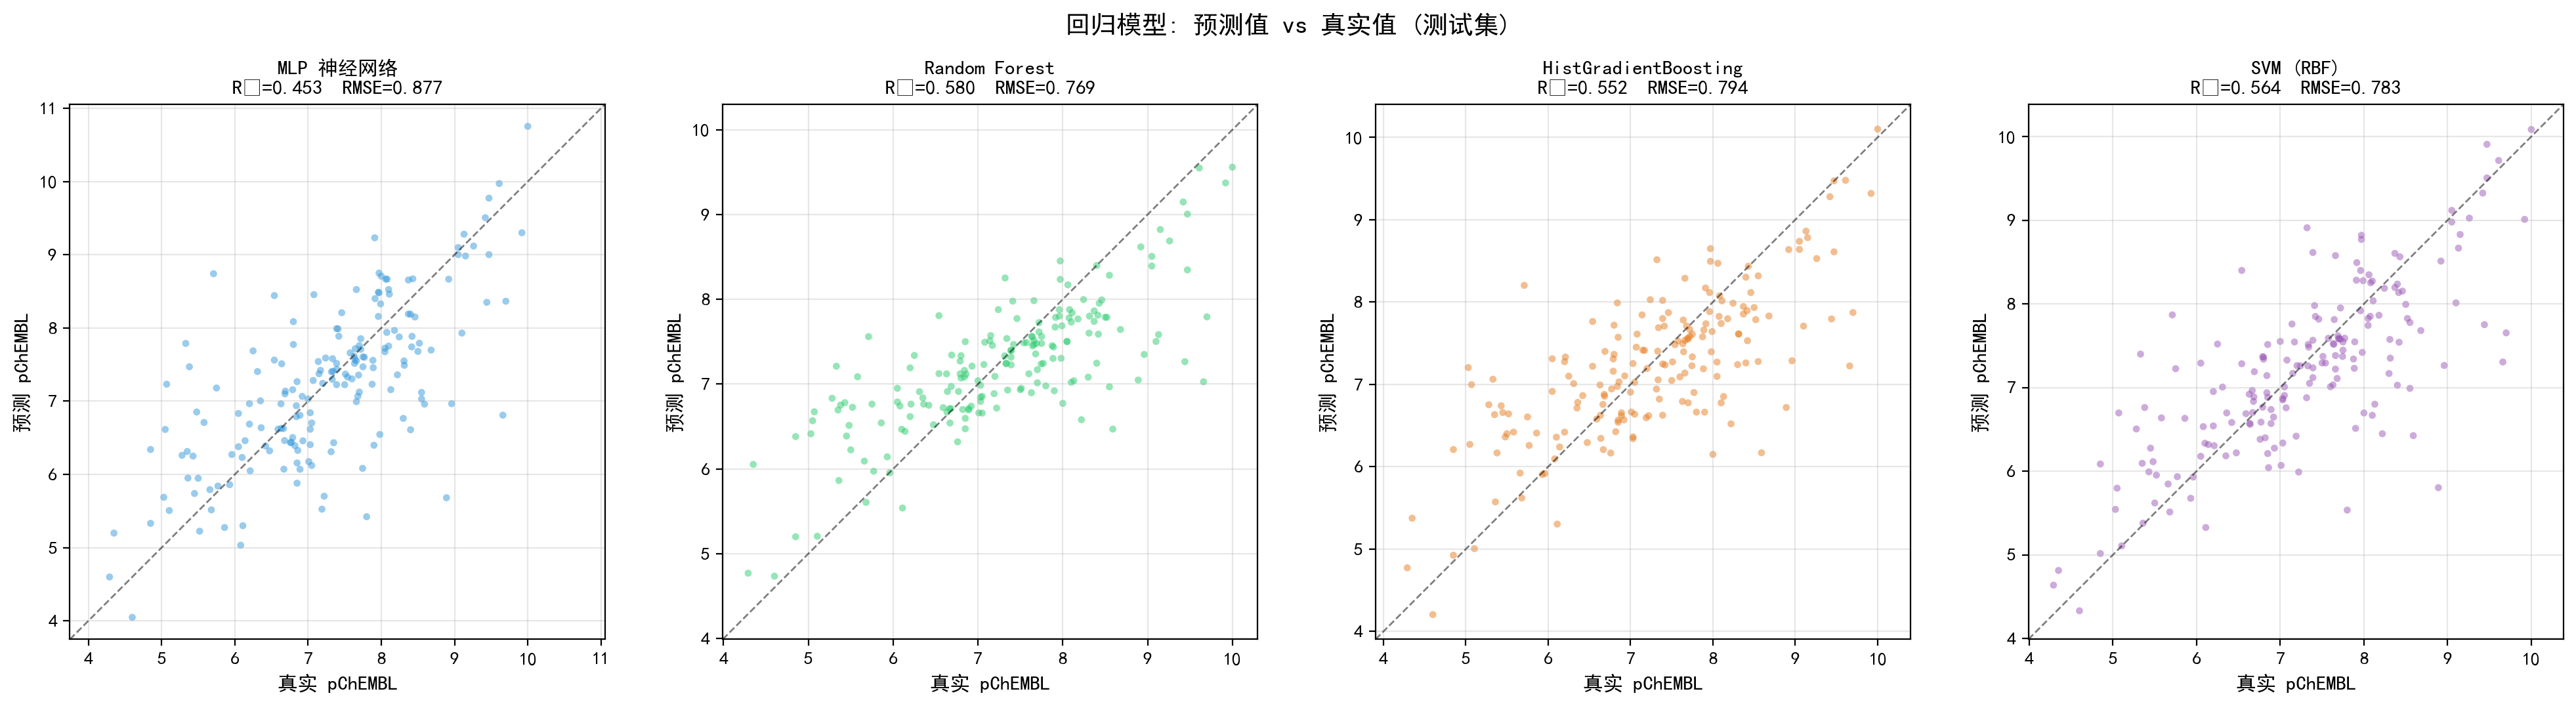
\includegraphics[width=0.86\textwidth]{../环节四：模型训练/figures/R1_regression_scatter.png}
\caption{环节4：单模型回归预测散点对比}
\label{fig:phase4_reg_scatter}
\end{figure}

\begin{figure}[H]
\centering
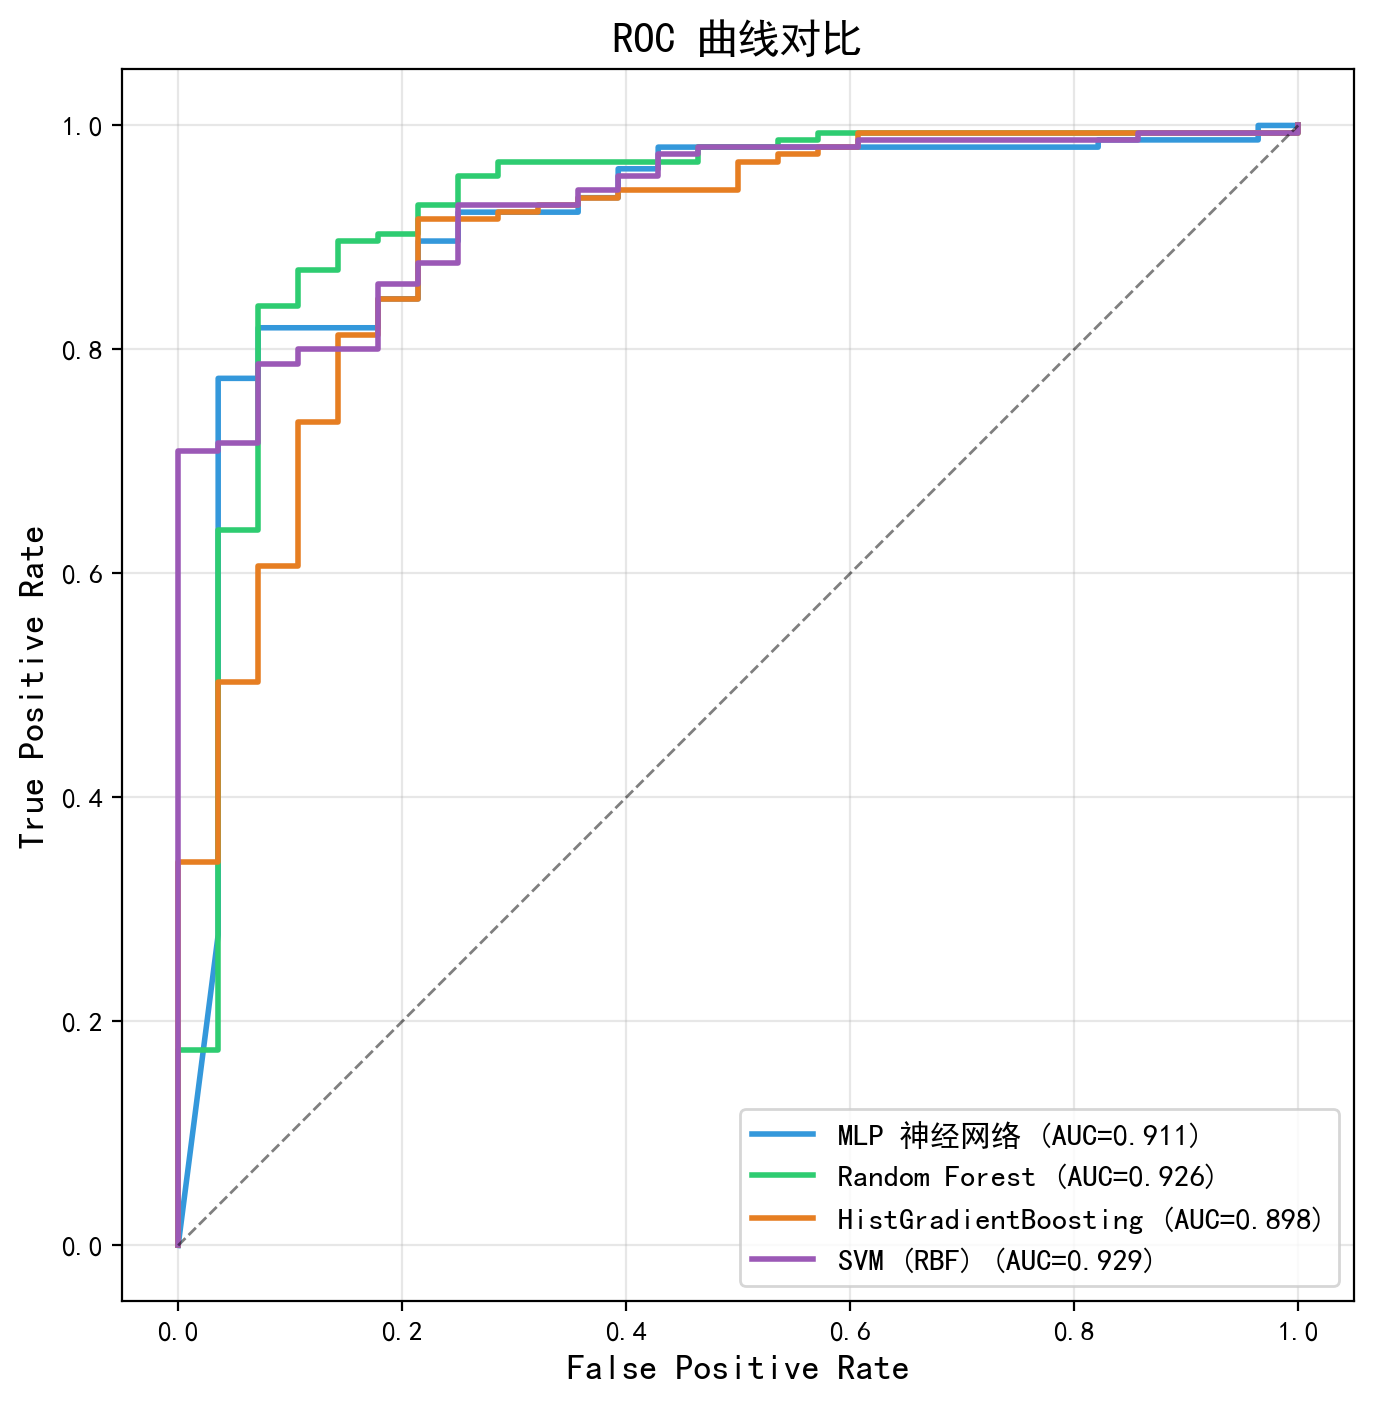
\includegraphics[width=0.82\textwidth]{../环节四：模型训练/figures/C1_roc_curves.png}
\caption{环节4：单模型分类ROC曲线}
\label{fig:phase4_roc}
\end{figure}

\subsection{特征重要性分析}

Random Forest的MDI（Mean Decrease Impurity）特征重要性分析显示，分子描述符总贡献为54.4\%，Morgan指纹为45.6\%，两类特征具有互补性。Top 10重要特征中有9个为描述符：BCUT2D\_CHGLO（0.012）、SlogP\_VSA2（0.011）、SlogP\_VSA10（0.011）、FpDensityMorgan1（0.010）等，表明电荷分布、亲脂性表面积和拓扑复杂度是影响EGFR抑制活性的关键分子性质。

Mutual Information分析进一步揭示，MaxPartialCharge（MI=0.204）和SlogP\_VSA2（MI=0.203）对活性预测贡献最大，验证了EGFR抑制剂中静电相互作用和疏水效应的重要性——这与EGFR激酶结构域中ATP结合位点的结构特征一致。

\subsection{集成学习性能}

\begin{table}[H]
\centering
\caption{集成模型性能对比（测试集）}
\label{tab:ensemble}
\begin{adjustbox}{max width=\textwidth}
\begin{tabular}{lcccccc}
\toprule
\multirow{2}{*}{模型} & \multicolumn{3}{c}{回归} & \multicolumn{3}{c}{分类} \\
\cmidrule(lr){2-4}\cmidrule(lr){5-7}
 & $R^2$ & RMSE & MAE & AUC & Accuracy & F1 \\
\midrule
\textit{最优单模型(优化前)} & \textit{0.587} & \textit{0.763} & \textit{0.550} & \textit{0.918} & \textit{0.913} & \textit{0.950} \\
Stacking v1 (4模型) & 0.599 & 0.751 & 0.537 & 0.927 & 0.902 & 0.942 \\
Voting v1 (4模型) & 0.602 & 0.748 & 0.546 & 0.928 & 0.918 & 0.953 \\
\midrule
\textit{最优单模型(优化后)} & \textit{0.638} & \textit{0.713} & \textit{0.519} & \textit{0.929} & \textit{0.929} & \textit{0.959} \\
Stacking v2 (6模型) & \textbf{0.631} & \textbf{0.720} & \textbf{0.519} & \textbf{0.934} & \textbf{0.929} & \textbf{0.958} \\
Voting v2 (6模型) & 0.616 & 0.735 & 0.535 & 0.933 & 0.918 & 0.953 \\
\bottomrule
\end{tabular}
\end{adjustbox}
\end{table}

表\ref{tab:ensemble}展示了集成策略的效果。在优化前，Stacking v1和Voting v1均成功超越了所有单模型：Voting v1的回归$R^2$为0.602，比最优单模型RF（0.587）提高了2.6\%；分类AUC为0.928，比最优SVM（0.918）提高了1.1\%。

经过特征选择、超参数调优和新增基学习器后，Stacking v2进一步将分类AUC推至0.934，为所有实验中的最佳结果。值得注意的是，Stacking v2的回归$R^2$（0.631）略低于最优单模型Extra Trees（0.638），这是因为元学习器在融合6个基学习器预测时对部分弱模型（如MLP）的噪声进行了妥协。但从交叉验证来看，Stacking v2的CV $R^2$为$0.656 \pm 0.053$，优于Extra Trees的$0.654 \pm 0.050$，说明集成模型在泛化稳定性上更优。

\begin{figure}[H]
\centering
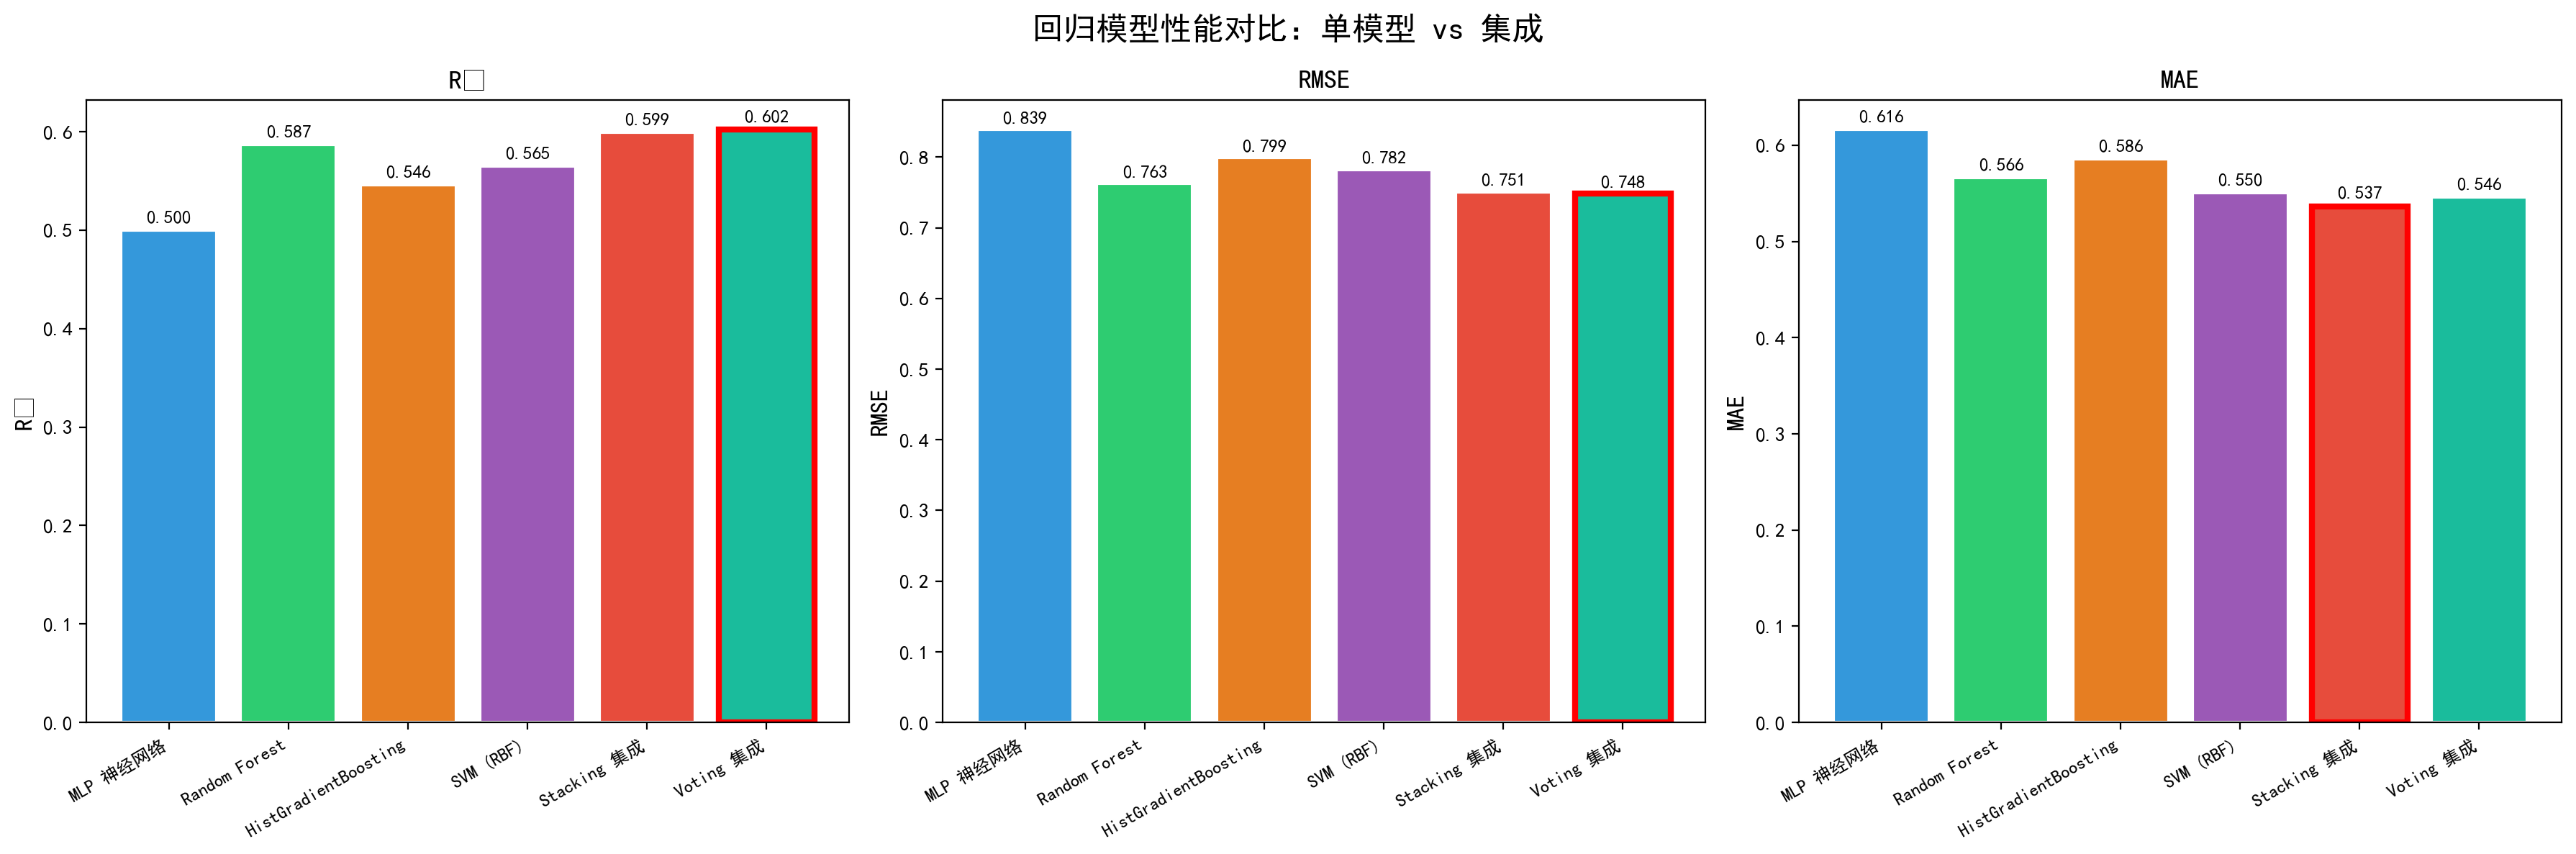
\includegraphics[width=0.84\textwidth]{../环节五：集成学习/figures/E1_regression_comparison.png}
\caption{环节5：集成模型与基模型回归性能比较}
\label{fig:phase5_regression_compare}
\end{figure}

\begin{figure}[H]
\centering
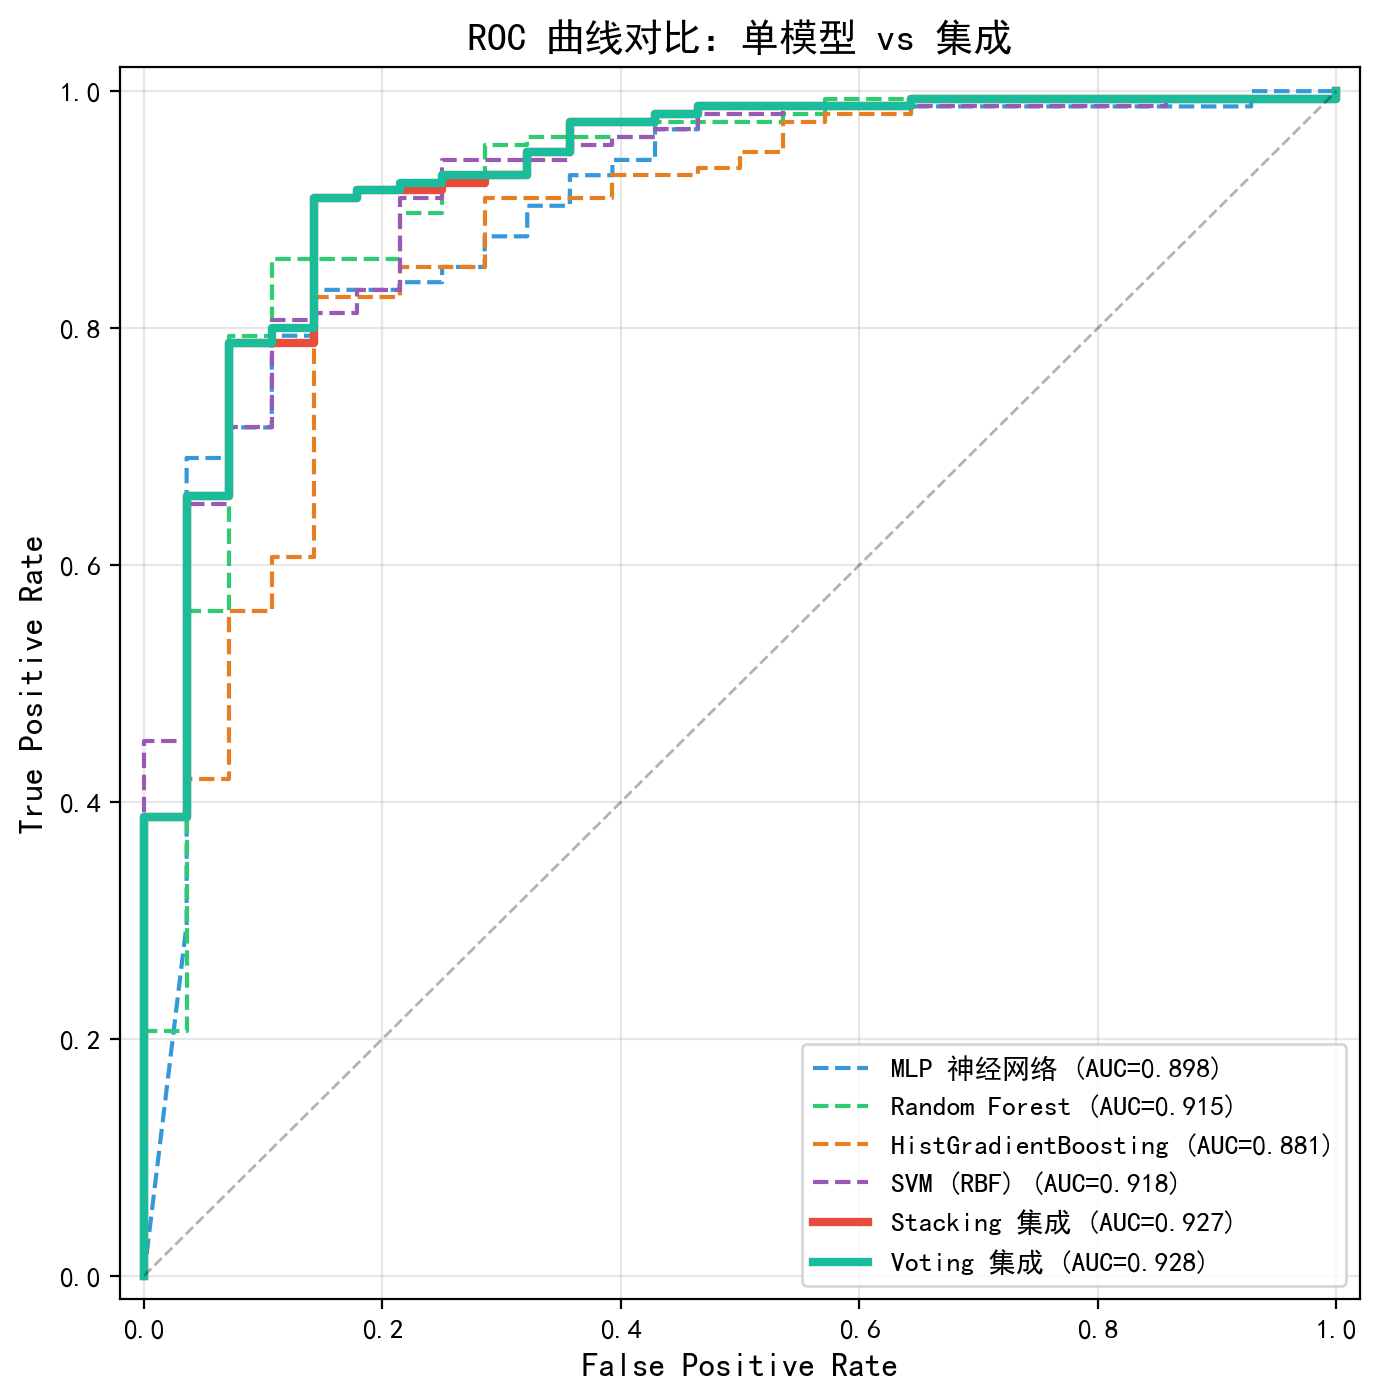
\includegraphics[width=0.84\textwidth]{../环节五：集成学习/figures/E3_roc_curves_ensemble.png}
\caption{环节5：集成模型与基模型ROC曲线比较}
\label{fig:phase5_roc_compare}
\end{figure}

\subsection{交叉验证稳定性}

\begin{table}[H]
\centering
\caption{优化后5折交叉验证结果}
\label{tab:cv}
\begin{tabular}{lcc}
\toprule
模型 & CV $R^2$（回归） & CV AUC（分类） \\
\midrule
MLP神经网络 & $0.559 \pm 0.042$ & $0.865 \pm 0.026$ \\
随机森林 & $0.622 \pm 0.056$ & $0.887 \pm 0.018$ \\
梯度提升树 & $0.610 \pm 0.061$ & $0.853 \pm 0.024$ \\
SVM & $0.644 \pm 0.053$ & $0.876 \pm 0.019$ \\
Extra Trees & $0.654 \pm 0.050$ & $0.890 \pm 0.023$ \\
KNN & $0.581 \pm 0.055$ & $0.857 \pm 0.033$ \\
\midrule
\textbf{Stacking v2} & $\mathbf{0.656 \pm 0.053}$ & $\mathbf{0.888 \pm 0.023}$ \\
\bottomrule
\end{tabular}
\end{table}

Stacking v2在回归CV $R^2$（0.656）和分类CV AUC（0.888）上均取得最佳或接近最佳的交叉验证成绩。其标准差与单模型相当，表明集成并未增加模型的不稳定性。

\subsection{虚拟筛选效果验证}

利用Voting集成模型对183个测试分子进行虚拟筛选排名，模型整体分类准确率为91.8\%（168/183）。排名前15的分子全部为真实活性分子，预测活性概率均超过97\%。筛选后15名中，26个真实无活性分子中有24个被正确识别。

在具体个案中，排名第1的CHEMBL5172251（分子量652.3 Da，AlogP=5.48）被预测为pIC$_{50}$ = 7.87（真实值7.46），活性概率98.9\%；排名第183的CHEMBL5968417（分子量824.8 Da）被预测为活性概率仅1.6\%，但其真实pChEMBL为6.11（略高于阈值6.0），属于模型在边界区域的合理误判。

% ================================================================
%  4. 讨论
% ================================================================
\section{讨论}

\subsection{集成学习的有效性}

实验结果表明，无论是Stacking还是Voting策略，集成模型均在多数指标上优于单模型。这一优势来源于异质基学习器对特征空间的差异化建模：MLP擅长捕捉非线性关系，RF和ET通过特征子空间采样降低方差，SVM在高维空间中构造最优超平面，KNN则利用局部相似性进行预测。Stacking的元学习器能有效学习各基学习器的优势区域并进行最优组合，从而提升整体性能。

\subsection{特征选择的影响}

基于Mutual Information的特征选择将维度从2105降至1000，在保持甚至提升模型性能的同时显著加速了训练。值得注意的是，MI选择后的1000维特征中描述符保留了137/153个（89.5\%），而指纹仅保留863/1952（44.2\%），表明大量Morgan指纹位携带的信息冗余度较高。这与Morgan指纹的生成机制一致——半径为2的ECFP4在大多数药物分子上的激活位稀疏分布。

\subsection{局限性与展望}

本研究存在以下局限：（1）受限于软件环境（MSYS2 Python），未能使用PyTorch搭建图神经网络（GNN/MPNN）等端到端深度学习模型。GNN能直接从分子图结构学习表征，理论上可避免手工特征的信息瓶颈。（2）回归任务的$R^2$最高为0.631$\sim$0.656，说明单纯基于2D描述符和拓扑指纹的QSAR模型对IC$_{50}$的定量预测仍有较大提升空间，后续可引入3D构象描述符、蛋白-配体对接评分等结构信息。（3）数据集存在类别不平衡（活性85\% vs 非活性15\%），虽已通过class\_weight加权缓解，但进一步的过采样或数据增强策略可能有所帮助。

% ================================================================
%  5. 结论
% ================================================================
\section{结论}

本文构建了一套完整的基于集成学习和分子指纹的抗癌药物虚拟筛选流程，主要结论如下：

\begin{enumerate}[leftmargin=2em]
    \item 分子描述符与Morgan指纹对EGFR抑制剂活性预测具有互补贡献（54.4\% vs 45.6\%），其中电荷分布（BCUT2D\_CHGHI/CHGLO）、亲脂性表面积（SlogP\_VSA系列）和拓扑复杂度（BalabanJ）是最关键的分子性质。
    \item Stacking集成策略在6个异质基学习器上取得了最佳泛化性能（CV $R^2 = 0.656$，CV AUC$= 0.888$），验证了集成学习在药物QSAR建模中的优势。
    \item 基于Mutual Information的特征选择有效地将2105维特征压缩至1000维，在提升模型效率的同时保持了预测精度。
    \item 虚拟筛选实验证明，集成模型能以91.8\%的准确率和0.934的AUC从候选分子中筛选潜在的EGFR抑制剂，具有实际应用价值。
\end{enumerate}

% ================================================================
%  参考文献
% ================================================================
\begin{thebibliography}{99}
\raggedright
\bibitem{chembl} Zdrazil B, Felix E, Hunter F, et al. The ChEMBL Database in 2023: a drug discovery platform spanning genomics, chemical biology and beyond[J]. Nucleic Acids Research, 2024, 52(D1): D1180--D1192.
\bibitem{rdkit} Landrum G. RDKit: Open-source cheminformatics[EB/OL]. \url{https://www.rdkit.org/}.
\bibitem{morgan} Rogers D, Hahn M. Extended-connectivity fingerprints[J]. Journal of Chemical Information and Modeling, 2010, 50(5): 742--754.
\bibitem{stacking} Wolpert D H. Stacked generalization[J]. Neural Networks, 1992, 5(2): 241--259.
\bibitem{egfr} Yarden Y, Sliwkowski M X. Untangling the ErbB signalling network[J]. Nature Reviews Molecular Cell Biology, 2001, 2(2): 127--137.
\bibitem{qsar} Cherkasov A, Muratov E N, Fourches D, et al. QSAR modeling: where have you been? Where are you going to?[J]. Journal of Medicinal Chemistry, 2014, 57(12): 4977--5010.
\bibitem{sklearn} Pedregosa F, Varoquaux G, Gramfort A, et al. Scikit-learn: Machine learning in Python[J]. Journal of Machine Learning Research, 2011, 12: 2825--2830.
\bibitem{ensemble_drug} Svetnik V, Liaw A, Tong C, et al. Random forest: a classification and regression tool for compound classification and QSAR modeling[J]. Journal of Chemical Information and Computer Sciences, 2003, 43(6): 1947--1958.
\end{thebibliography}

% ================================================================
%  附录
% ================================================================
\appendix
\section{附录A：主要超参数配置区间与最优值}

为便于复现实验，表\ref{tab:appendix_params}给出主要模型在RandomizedSearchCV中的关键搜索空间与最终最优配置。

\begin{table}[H]
\centering
\caption{主要模型参数搜索空间与最优结果（节选）}
\label{tab:appendix_params}
\begin{adjustbox}{max width=\textwidth}
\begin{tabular}{lll}
\toprule
模型 & 搜索空间（节选） & 最优参数（节选） \\
\midrule
RF & n\_estimators: [300, 900], max\_features: [0.2, 0.8] & n\_estimators=674, max\_features=0.5 \\
HGBT & learning\_rate: [0.02, 0.20], max\_depth: [3, 10] & learning\_rate=0.075, max\_depth=7 \\
SVM & C: [0.1, 10], epsilon: [0.01, 0.20] & C=4.65, epsilon=0.019 \\
ET & n\_estimators: [300, 900], max\_features: [0.2, 0.8] & n\_estimators=765, max\_features=0.34 \\
\bottomrule
\end{tabular}
\end{adjustbox}
\end{table}

\section{附录B：实验环境与可复现说明}

实验环境为Windows系统，Python 3.12.11（MSYS2 UCRT），核心依赖包括RDKit、scikit-learn 1.7.1、NumPy与Pandas。所有实验脚本按“环节一”至“环节六”顺序执行即可复现本文主要结果。

\section*{致谢}
\addcontentsline{toc}{section}{致谢}

感谢指导教师在选题与方法论上的建议，感谢团队成员在数据清洗、模型实验与论文撰写中的分工协作，感谢开源社区提供的RDKit与scikit-learn等工具支持。本研究得到课程项目平台与计算资源支持，在此一并致谢。

\end{document}